
\documentclass[conference]{IEEEtran}
\usepackage{blindtext}
\usepackage{graphicx}
\usepackage{listings}
\usepackage[portuges, brazil]{babel}
\usepackage[utf8]{inputenc}
\usepackage{hyperref}
\usepackage{booktabs}
\usepackage{esdiff}
\usepackage{amsmath}
%\usepackage{authblk} to multiple authors
\usepackage[hang, small,labelfont=bf,up,textfont=it,up]{caption}


\ifCLASSINFOpdf
\else
\fi


\hyphenation{op-tical net-works semi-conduc-tor}


\begin{document}
\title{Implementação de um Controlador Fuzzy para um sistema de tanques acoplados: um estudo de caso.}
\author{\IEEEauthorblockN{Fernando Leandro Fernandes}\IEEEauthorrefmark{1},Rosenildo Furtado\IEEEauthorrefmark{2} e Tiago Batista S. Sousa\IEEEauthorrefmark{3}
\IEEEauthorblockA{Universidade Federal do Rio Grande do Norte\\Departamento de Engenharia de Computação e Automação\\Natal, Rio Grande do Norte\\Email:\IEEEauthorrefmark{1}leandes@gmail.com,\IEEEauthorrefmark{2}reidesgm@hotmail.com,\IEEEauthorrefmark{3}ekyidag@gmail.com}}

\maketitle


\begin{abstract}
Este estudo aborda de configuração de um controlador PI nebuloso utilizando os modelos de Sugeno e Mamdani para o controle de um sistema de tanques acoplados. Esta atividade foi desenvolvida utilizando o toolbox Fuzzy do Matlab R2016a Student e um modelo fornecido do Simulink. O objetivo do estudo é obter parâmetros de operação ótimos para o controlador PI dadas as condições de operação, considerando como entradas o erro entre o setpoint e o nível presente na planta e a variação(derivada) desse erro. Esta atividade foi proposta pelo Prof. Dr. Fábio Meneghetti no escopo do componente Controle Fuzzy de Sistemas Dinâmicos do curso de Engenharia Mecatrônica da Universidade Federal do Rio Grande do Norte.

\end{abstract}
\begin{IEEEkeywords}
Controle PI nebuloso, Lógica nebulosa, Controle proporcional-integrativo
\end{IEEEkeywords}
\IEEEpeerreviewmaketitle


\section{Introdução}

A teoria dos conjuntos nebulosos, idealizada em 1965 pelo matemático e pesquisador das área de ciência da computação, engenharia elétrica e inteligência artificial, o azerbaijano Lotfali Askar-Zadeh, é o alicerce da teoria que modela sistemas que lidam com dados e regras imprecisas. Assim como as pessoas o fazem cotidianamente.

A partir desse conceito, todo um conjunto de técnicas e tecnologias que fazem uso de definições linguísticas para o tratamento das informações e das ações de controle foi desenvolvida e estão presentes virtualmente em qualquer aparelho que necessite realizar inferências de controle mais refinadas que o simples controle \textit{on/off}.

Controladores nebulosos atualmente ocupam posição de destaque entre as técnicas de controle empregadas na indústria, ficando atrás apenas do controle PID clássico.

\section{Referencial Teórico}

Nesta seção discutiremos aspectos teóricos relacionados à implementação do nosso projeto de controle. A lógica nebulosa permite tratarmos, com mais precisão, situações onde a lógica tradicional não se faz eficiente(quando variáveis linguísticas entram em análise). Ela se baseia na teoria dos conjuntos nebulosos.

As primeiras aplicações de algoritmos \textit{fuzzy} em problemas de controle foi trabalho pioneiro de Mamdani(1973), seguido por Sugeno(1985), ambos motivados pelos trabalhos de Zadeh(1965 e 1973). Sugeno, observando dificuldades para a implementação do processo de decisão do controlador de Mamdani, propôs um método de tomada de decisão simplificado, baseado na lógica \textit{fuzzy}, onde somente o antecedente das regras é formado por variáveis \textit{fuzzy}. O conseqüente de cada regra é expresso por uma função linear dos valores observados das variáveis que descrevem o estado do sistema (variáveis de entrada). Este tipo de controlador é referido na literatura como controlador de Sugeno (Lee, 1990a; Zimmermann, 1996; MathWorks, 2008).


\subsection{Conjuntos Nebulosos}

Diferentemente da teoria clássica de conjuntos, na qual um elemento pode pertencer ou não a um determinado conjunto, a teoria dos conjuntos nebulosos quebra esse paradigma, definindo o que se chama de funções de pertinência. Essas funções assumem valores de 0 a 1, significando que um certo elemento pertence de 0 a 100\% àquele conjunto A, cuja função de pertinência é $\mu_A(x)$. Um exemplo está na figura 1.

\begin{figure}[!ht]
    %figura 1
    \centering
    \includegraphics[scale=0.75]{ex_fp.png}
    \caption { Exemplo de função de pertinência($\mu_A(x)$) de um elemento x a um conjunto hipotético A, quando esse elemento abrange valores de zero a cinco. }
\end{figure}

Essa teoria se mostra particularmente eficiente ao tratarmos casos onde a transição dos valores de pertinência a certos conjuntos devem ser contínuos, como uma pessoa com febre. Seja $F$ o conjunto das pessoas que estão com febre, comumente dizemos que até 37,8ºC, o indivíduo $x$ não participa desse conjunto($\mu_F(x) = 0$) e a partir desse valor, participa desse contjunto($\mu_F(x) = 1$). Obviamente essa descrição não é boa, pois trata por igual aqueles que tem graus de febre diferentes. Neste exemplo, temos a seguinte situação, descrita pelas equações 1 e 2, como também pela figura 2:

\begin{equation}
\mu_F(x) = 0; \forall x < 37.8 ºC
\end{equation}

\begin{equation}
\mu_F(x) = 0; \forall x \geq 37.8 ºC
\end{equation}

\begin{figure}[!ht]
    %figura 2
    \centering
    \includegraphics[scale=1]{mi_feb.png}
    \caption { Exemplo de função de pertinência clássica($\mu_F(x)$,x) de um elemento temperatura ao conjunto F. }
\end{figure}

\section{Desenvolvimento}

Controladores aprimorados de Mamdani e Sugeno têm sido utilizados para diferentes aplicações (Lee, 1990a). Atualmente estão disponíveis em pacotes computacionais, com diferentes recursos para implementação dos seus componentes, o que facilita o desenvolvimento de controladores \textit{fuzzy} para a solução de diferentes problemas de controle. A escolha do tipo de controlador a adotar e a forma de implementação dos seus diferentes componentes, exige do projetista conhecimento dos aspectos teóricos envolvidos em cada solução e, além disso, razoável noção do impacto de cada escolha (tipo de controlador e implementação dos componentes) sobre a eficácia do controle por ele produzido.

No controlador desenvolvido foi adotado um método para o processo de decisão baseado em regras do tipo “SE A ENTÃO B”, nas quais tanto o antecedente quanto o conseqüente são valores de variáveis lingüísticas, expressos por meio de conjuntos \textit{fuzzy} (Mamdani e Assilian, 1975). 

Os controladores fuzzy são classificados em função do seu método de tomada de decisão e podem ser reunidos em dois grandes grupos. O primeiro(modelo Mamdani),  define funções de pertinência para os conjuntos saída e  aplicam um dos métodos de defuzificação(explicados mais a frente)  para  obter o sinal de controle $u(k)$. Já os do segundo(modelo Sugeno), dispensa a definição de funções de pertinência para os conjuntos de saída e a utilizam como função das entradas. Tendo como entradas do controlador os sinais a e b, podemos dizer que o sinal de controle: $u(k)$ $=$ $f(a,b)$.

Nos dois tipos de controladores a ação de controle é obtida por meio da definição de um conjunto de instruções (ou regras) de controle. A tabela <inserir numero> mostra um exemplo de regras de controle.

\begin{table}[!ht]
\caption{Exemplo de regras para um controlador fuzzy de duas entradas,  com três funções de pertinência para cada uma delas - note que as regras podem se repetir em diferentes combinações de entradas, quando necessário}
\centering
\begin{tabular}{lllr}
\toprule
\multicolumn{3}{r}{\textbf{$e(k)$}} \\
\cmidrule(r){2-4}
\textbf{$\Delta$e(k)} & \textbf{Negativo} & \textbf{Nulo} & \textbf{Positivo} \\
Negativo & $R_1$ & $R_2$ & $R_3$ \\
Nulo & $R_4$ & $R_5$ & $R_6$ \\
Positivo & $R_7$ & $R_8$ & $R_9$ \\
\bottomrule
\end{tabular}
\end{table}

\subsection{Controlador Mamdani}

A ação deste controlador é definida pela agregação das n regras $R_i$ que foram ativadas pelas entradas do algoritmo. Esta agregação resulta numa função de pertinência do conjunto fuzzy de saída C($\mu_C(x)$). A saída efetiva do controlador(valor numérico) é então obtida por meio de um processo de defuzificação aplicado ao conjunto C. 


\subsubsection{Métodos de defuzificação - Centro de área(CoA)}

O método do centro de área é calculado tomando o centro geométrico da função de pertinência do conjunto de saída C($\mu_C(x)$) do controlador nebuloso. Apesar de oferecer os melhores resultados, ele não é muito utilizado pois requer alto esforço computacional.

\subsubsection{Métodos de defuzificação - Média dos máximos(MoM)}

Tomando os valores de máximo da função $\mu_C(x)$ e tirando a média, podemos obter uma boa aproximação para o valor numérico oferecido pelo método do centro de área sem a necessidade de um esforço computacional tão elevado.


\subsection{Controlador Sugeno}

O controlador de Sugeno é uma versão simplificada do controlador de Mamdani, onde o conseqüente de cada regra é definido como uma função das variáveis lingüísticas de entrada. Isto é, sejam x(k) e y(k) as entradas do controlador nebuloso e z sua saída, a regra geral $R_i$ pode ser escrita como:\\
Regra($R_i$): se $x$ é $A_i$ e y é $B_i$ então $z$ $=$ $f_i(x,y)$\\
A equação 1 exemplifica uma função de sugeno bilinear(sistema com duas entradas), com coeficientes a, b e c.

\begin{equation}
%\label{eq:dL1}
z(k) = f(x(k),y(k)) = ax(k) + by(k) + c
\end{equation}

Podemos observar que o resultado da regra  é um valor numérico, resultado do cálculo da função de sugeno z naquele momento. Dessa forma, fica dispensada a definição de uma função de inferência. Realizando uma média ponderada de todas as funções $f_i$ ativadas por cada regra $R_i$, obtemos o valor numérico de saída do controlador. Ou seja, não há processo de defuzificação no controlador Sugeno.
1
\subsection{Implementação computacional} AQUI!

Atualmente, alguns programas de uso geral dispõem de módulos específicos para facilitar a implementação computacional de um sistema de controle nebuloso, como é o caso do \textit{Fuzzy Logic Toolbox} do \textit{MATLAB}\textsuperscript{\textregistered}, usado neste trabalho para implementar os dois tipos de controladores em estudo. O programa permite ao usuário definir os componentes principais do sistema de controle, que são: fuzificação dos valores das variáveis de entrada(definição das funções de pertinência das entradas aos conjuntos fuzzy escolhidos - ver tabela 1) e aplicação dos operadores que podem estar presentes no antecedente das regras (“e” e “ou”); funções de implicação para o conjunto de saída C; agregação dos conseqüentes de todas as regras definidas; e o método de defusificação do conjunto de saída C. No MATLAB\textsuperscript{\textregistered}, antes de iniciar a definição dos componentes do sistema, o usuário deve indicar se o seu controlador é do tipo Mamdani ou Sugeno. Dependendo do tipo selecionado, são liberados os campos pertinentes para a entrada dos dados. Isto é, se for selecionado o controlador de Sugeno, por exemplo, os campos referentes à função de implicação, ao termo de agregação “também” e ao método de defuzificação ficam desabilitados. O programa apresenta diferentes opções ao usuário para a configuração dos componentes do sistema e, para a maioria dos campos, também permite a definição de outras alternativas.

\subsection{O problema}

O sistema a ser controlado é o sistema de tanques acoplados da Quanser, que tem model matemático dado por:
\begin{equation}
\label{eq:dL1}
\dot{L_{1}} = - \frac{a_{1}}{A_{1}} \sqrt{\frac{g}{2L_{1o}}}L_{1}+\frac{K_{m1}}{A_{1}}V_{p1}
\end{equation}

\begin{equation}
\label{eq:dL2}
\dot{L_{2}} = - \frac{a_{2}}{A_{2}} \sqrt{\frac{g}{2L_{2o}}}L_{2}+\frac{a_{1}}{A_{1}} \sqrt{\frac{g}{2L_{1o}}}L_{1}
\end{equation}

Onde $L_{1}$ e $\dot{L_{1}}$ são o nível do tanque superior e sua variação. O mesmo vale para $L_{2}$ e $\dot{L_{2}}$, para o tanque inferior; $a_{1}$ e $A_{1}$, assim como $a_{2}$ e $A_{2}$, são as áreas dos orifícios e da seção transversal dos tanques superior e inferior, respectivamente. $V_{p1}$ é a tensão aplicada à bomba e $K_{m1}$ é a constante da bomba. Discretizando o modelo para o período de amostragem da planta (100 ms) e aplicando as constantes fornecidas pelo fabricante do experimento temos:

\begin{equation}
\label{eq:discrete}
\begin{cases}
L_{1}(k) = 0,9935 L_{1}(k-1) + 0,0296V_{p1}(k-1) \\
L_{2}(k) = 0,0065L_{1}(k-1)+0,9935L_{2}(k-1)+ \\ 
\hspace{1.33cm}0,0001V_{p1}(k-1)
\end{cases}
\end{equation}

\section{Metodologia}

A partir da simulação representada na figura 3, realizamos a sintonia de controladores fuzzy do tipo Mamdani e Sugeno.

De forma suscinta, as funções de pertinência foram incialmente escolhidas empiricamente e refinadas conforme foram sendo realizadas as simulações e observado o comportamento do sistema. Baseado nas funções de pertinência definidas foi construída o conjunto de regras de inferência, considerando a quantidade de entradas e funções. Em sequência, definiram-se as funções lineares de pertinência da saída, a saber:

\itemize{
\item{MANTER: ação fraca para manutenção do nível do tanque quando nível está próximo ao \textit{setpoint}.}
\item{SUBIR: ação moderada para aumento do nível do tanque quando o nível do tanque está abaixo do \textit{setpoint}, mas convergindo para ele.}
\item{DESCER: ação moderada para redução do nível do tanque quando o nível do tanque está acima do \textit{setpoint}, mas convergindo para ele.}
\item{SUBIR FORTE: ação intensa para aumento do nível do tanque quando o nível está divergindo decrescentemente do \textit{setpoint}.}
\item{DESCER FORTE: ação intensa para redução do nível do tanque quando o nível está divergindo crescentemente do \textit{setpoint}.}
}

O parâmetros de controle definidos para cada umas das funções de saída, expresso por um vetor de saída com 3 elementos, onde o primeiro comporta-se como o fator integrativo, o segundo como o proporcional e o terceiro como uma constante de offset do modelo clássico da teoria de controle. Os valores foram escolhidos pela observação do comportamento da simulação.

\begin{figure}[!ht]
    %figura 2
    \centering
    \includegraphics[scale=0.4]{simul.png}
    \caption { Simulação do sistema de controle \textit{fuzzy} utilizado. }
\end{figure}

\section{Resultados}

\subsection{Mamdani - melhor resultado}

As tabelas 2, 3, 4  e 5 representam respectivamente, as regras para o controlador Mamdani, os parâmetros de pertinência para a entrada $e(k)$, os parâmetros de pertinência  para a entrada $\Delta$e(k) e os parâmetros de inferência de saída $u(k)$, enquanto a figura 4 mostra o comportamento do nível do tanque 2(variável manipulada) em relação ao nosso referencial

\begin{table}[!ht]
\caption{Regras do melhor controlador Mamdani encontrado}
\centering
\begin{tabular}{lllr}
\toprule
\multicolumn{3}{r}{\textbf{$e(k)$}} \\
\cmidrule(r){2-4}
\textbf{$\Delta$e(k)} & \textbf{Negativo} & \textbf{Nulo} & \textbf{Positivo} \\
Negativo & Descer & Descer & Subir \\
Nulo & Descer & Manter & Subir \\
Positivo & Descer & Subir & Subir \\
\bottomrule
\end{tabular}
\end{table}

\begin{table}[!ht]
\caption{Parâmetros de pertinência do erro para Mamdani}
\centering
\begin{tabular}{lr}
\toprule
\multicolumn{2}{c}{$e(k)$} \\
\cmidrule(r){1-2}
Negativo & [-54 -30 -3] \\
Nulo & [-5 -2.2 0.5] \\
Positivo & [-2 30 54] \\
\bottomrule
\end{tabular}
\end{table}

\begin{table}[!ht]
\caption{Parâmetros de pertinência da variação do erro para Mamdani}
\centering
\begin{tabular}{lr}
\toprule
\multicolumn{2}{c}{$\Delta$e(k)} \\
\cmidrule(r){1-2}
Negativo & [-1.8 -1 0] \\
Nulo & [-0.2 -0 0.2] \\
Positivo & [0 1 1.8] \\
\bottomrule
\end{tabular}
\end{table}

\begin{table}[!ht]
\caption{Parâmetros de inferência de saída para Mamdani}
\centering
\begin{tabular}{lr}
\toprule
\multicolumn{2}{c}{$e(k)$} \\
\cmidrule(r){1-2}
Descer & [-4 -2 -1] \\
Manter & [-1 -0 1] \\
Subir & [1 2 4] \\
\bottomrule
\end{tabular}
\end{table}

\begin{figure}[!ht]
    %figura 2
    \centering
    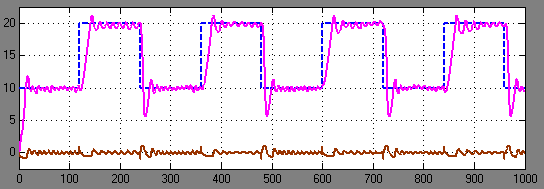
\includegraphics[scale=0.2]{mamdani1.png}
    \caption { Melhor resultado para o controlador do tipo Mamdani. }
\end{figure}

\subsection{Sugeno - melhor resultado}

As tabelas 6, 7, 8 e 9 representam respectivamente, as regras para o controlador Sugeno, os parâmetros de pertinência para a entrada $e(k)$, os parâmetros de pertinência  para a entrada $\Delta$e(k) e os parâmetros de inferência de saída $u(k)$, enquanto a figura 5 mostra o comportamento do nível do tanque 2(variável manipulada) em relação ao nosso referencial.

\begin{table}[!h]
\caption{Regras do melhor controlador Sugeno encontrado}
\centering
\begin{tabular}{lllr}
\toprule
\multicolumn{3}{r}{\textbf{$e(k)$}} \\
\cmidrule(r){2-4}
\textbf{$\Delta$e(k)} & \textbf{Negativo} & \textbf{Nulo} & \textbf{Positivo} \\
Negativo & $D_f$ & M & S \\
Nulo & D & M & S \\
Positivo & D & M & $S_f$ \\
\bottomrule
\end{tabular}
\end{table}

\begin{table}[!h]
\caption{Parâmetros de pertinência do erro para Sugeno}
\centering
\begin{tabular}{lr}
\toprule
\multicolumn{2}{c}{$e(k)$} \\
\cmidrule(r){1-2}
Negativo & [-4970 -4970 -8 -1] \\
Nulo & [-3 0 1] \\
Positivo & [0 6 30 5500] \\
\bottomrule
\end{tabular}
\end{table}

\begin{table}[!h]
\caption{Parâmetros de pertinência da variação do erro para Sugeno}
\centering
\begin{tabular}{lr}
\toprule
\multicolumn{2}{c}{$\Delta$e(k)} \\
\cmidrule(r){1-2}
Negativo & [-2 -1 0.104] \\
Nulo & [-0.2 0 0.1] \\
Positivo & [0 1 2] \\
\bottomrule
\end{tabular}
\end{table}

\begin{table}[!h]
\caption{Parâmetros das funções bilineares de saída para Sugeno}
\centering
\begin{tabular}{lr}
\toprule
\multicolumn{2}{c}{$\Delta$e(k)} \\
\cmidrule(r){1-2}
Descer Forte & [0.1 10 0] \\
Descer & [0.09 1.5 0] \\
Manter & [0.05 1 0] \\
Subir & [0.08 3 0] \\
Subir Forte & [0.05 2.5 0] \\
\bottomrule
\end{tabular}
\end{table}

\begin{figure}[!h]
    %figura 2
    \centering
    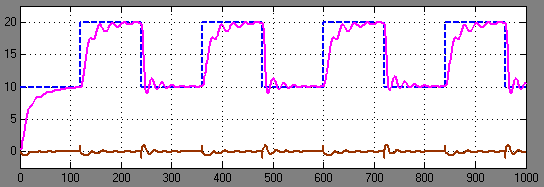
\includegraphics[scale=0.2]{sugeno1.png}
    \caption { Melhor resultado para o controlador do tipo Sugeno. }
\end{figure}

\subsection{Outros testes - Mamdani}

Esta seção abordará outros testes, realizados usando diferentes configurações Mamdani. As regras de controle foram mantidas as mesmas, alterando apenas os valores para funções de pertinência e inferência.

\begin{table}[!h]
\caption{Parâmetros de pertinência do erro para Mamdani - 2}
\centering
\begin{tabular}{lr}
\toprule
\multicolumn{2}{c}{$e(k)$} \\
\cmidrule(r){1-2}
Negativo & [-540 -10 -1] \\
Nulo & [-2 0 2] \\
Positivo & [1 10 540] \\
\bottomrule
\end{tabular}
\end{table}

\begin{table}[!h]
\caption{Parâmetros de pertinência da variação do erro para Mamdani - 2}
\centering
\begin{tabular}{lr}
\toprule
\multicolumn{2}{c}{$\Delta$e(k)} \\
\cmidrule(r){1-2}
Negativo & [-10 -1 -0.1] \\
Nulo & [-0.2 -0 0.2] \\
Positivo & [0 1 10.8] \\
\bottomrule
\end{tabular}
\end{table}

\begin{table}[!h]
\caption{Parâmetros de inferência de saída para Mamdani - 2}
\centering
\begin{tabular}{lr}
\toprule
\multicolumn{2}{c}{$e(k)$} \\
\cmidrule(r){1-2}
Descer & [-8 -2 -1] \\
Manter & [-1 -0 1] \\
Subir & [1 2 4] \\
\bottomrule
\end{tabular}
\end{table}

\begin{figure}[!h]
    %figura 2
    \centering
    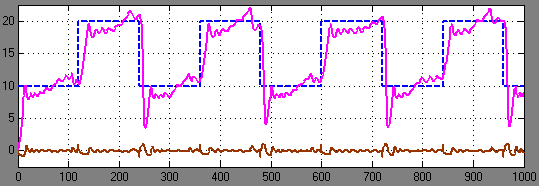
\includegraphics[scale=0.2]{mamdani2.png}
    \caption { Resultado para o controlador do tipo Mamdani - 2}
\end{figure}


\begin{table}[!h]
\caption{Parâmetros de pertinência do erro para Mamdani - 3}
\centering
\begin{tabular}{lr}
\toprule
\multicolumn{2}{c}{$e(k)$} \\
\cmidrule(r){1-2}
Negativo & [-540 -20 -2] \\
Nulo & [-3.5 -1 1] \\
Positivo & [0 10 540] \\
\bottomrule
\end{tabular}
\end{table}

\begin{table}[!h]
\caption{Parâmetros de pertinência da variação do erro para Mamdani - 3}
\centering
\begin{tabular}{lr}
\toprule
\multicolumn{2}{c}{$\Delta$e(k)} \\
\cmidrule(r){1-2}
Negativo & [-10 -1 0.01] \\
Nulo & [-0.2 -0 0.2] \\
Positivo & [0.01 1 10.8] \\
\bottomrule
\end{tabular}
\end{table}

\begin{table}[!h]
\caption{Parâmetros de inferência de saída para Mamdani - 3}
\centering
\begin{tabular}{lr}
\toprule
\multicolumn{2}{c}{$e(k)$} \\
\cmidrule(r){1-2}
Descer Forte & [-12 -4 1] \\
Descer & [-2 -1.5 -0.1] \\
Manter & [-0.6 0.1 0.5] \\
Subir & [0.1 1.25 2.25] \\
Subir Forte & [1 4 12] \\
\bottomrule
\end{tabular}
\end{table}

\begin{figure}[!h]
    %figura 2
    \centering
    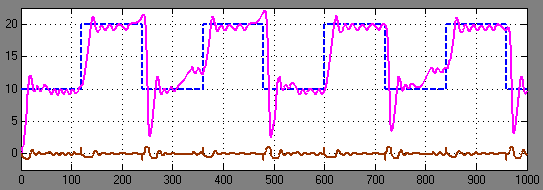
\includegraphics[scale=0.2]{mamdani3.png}
    \caption { Resultado para o controlador do tipo Mamdani - 3}
\end{figure}

\subsection{Outros testes - Sugeno}

Esta seção abordará outros testes, realizados usando diferentes configurações Sugeno. As regras de controle foram mantidas as mesmas, alterando apenas os valores para funções de pertinência e parâmetros das funções bilineares.

\begin{table}[!h]
\caption{Parâmetros de pertinência do erro para Sugeno - 2}
\centering
\begin{tabular}{lr}
\toprule
\multicolumn{2}{c}{$e(k)$} \\
\cmidrule(r){1-2}
Negativo & [-4970 -4970 -10 -1] \\
Nulo & [-5 0 5] \\
Positivo & [1 10 30 5500] \\
\bottomrule
\end{tabular}
\end{table}

\begin{table}[!h]
\caption{Parâmetros de pertinência da variação do erro para Sugeno - 2}
\centering
\begin{tabular}{lr}
\toprule
\multicolumn{2}{c}{$\Delta$e(k)} \\
\cmidrule(r){1-2}
Negativo & [-2 -1 0.104] \\
Nulo & [-0.2 0 0.2] \\
Positivo & [0 1 2] \\
\bottomrule
\end{tabular}
\end{table}

\begin{table}[!h]
\caption{Parâmetros das funções bilineares de saída para Sugeno - 2}
\centering
\begin{tabular}{lr}
\toprule
\multicolumn{2}{c}{$\Delta$e(k)} \\
\cmidrule(r){1-2}
Descer Forte & [0.5 10 0] \\
Descer & [0.18 3 0] \\
Manter & [0.04 0.55 0] \\
Subir & [0.08 2 0] \\
Subir Forte & [0.05 2.5 0] \\
\bottomrule
\end{tabular}
\end{table}

\begin{figure}[!h]
    %figura 2
    \centering
    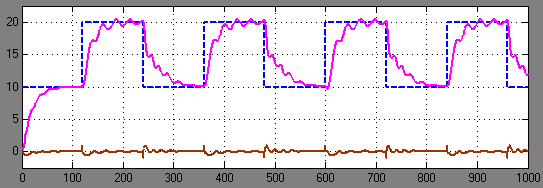
\includegraphics[scale=0.2]{sugeno3.png}
    \caption { Resultado para o controlador do tipo Sugeno - 2 }
\end{figure}

\begin{table}[!h]
\caption{Parâmetros de pertinência do erro para Sugeno - 3}
\centering
\begin{tabular}{lr}
\toprule
\multicolumn{2}{c}{$e(k)$} \\
\cmidrule(r){1-2}
Negativo & [-543 -87 -15 -3.5] \\
Nulo & [-5 1.15 3] \\
Positivo & [2 15 87 543] \\
\bottomrule
\end{tabular}
\end{table}

\begin{table}[!h]
\caption{Parâmetros de pertinência da variação do erro para Sugeno - 3}
\centering
\begin{tabular}{lr}
\toprule
\multicolumn{2}{c}{$\Delta$e(k)} \\
\cmidrule(r){1-2}
Negativo & [-10 -1 -0.08] \\
Nulo & [-0.15 0 0.08] \\
Positivo & [0.06 1 5] \\
\bottomrule
\end{tabular}
\end{table}

\begin{table}[!h]
\caption{Parâmetros das funções bilineares de saída para Sugeno - 3}
\centering
\begin{tabular}{lr}
\toprule
\multicolumn{2}{c}{$\Delta$e(k)} \\
\cmidrule(r){1-2}
Descer Forte & [0.5 10 0] \\
Descer & [0.3 10 0] \\
Manter & [0.045 1.7 0] \\
Subir & [0.19 6.5 0] \\
Subir Forte & [0.25 3.8 0] \\
\bottomrule
\end{tabular}
\end{table}

\begin{figure}[!h]
    %figura 2
    \centering
    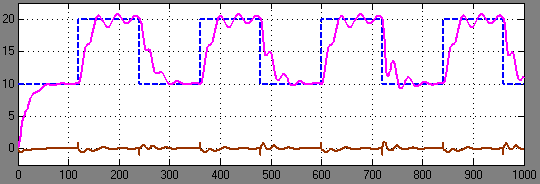
\includegraphics[scale=0.2]{sugeno2.png}
    \caption { resultado para o controlador do tipo Sugeno - 3 }
\end{figure}

\ifCLASSOPTIONcaptionsoff
  \newpage
\fi

\section{Conclusões}

Analisando as figuras 4 e 5, podemos observar que,  apesar de mais complexo, o controlador Mamdani reagiu melhor ao sistema, com um tempo de acomodação consideravelmente melhor. Entretanto, este apreseta um valor de \textit{overshoot}, que é menor nos controladores Sugeno. Além disso, o controlador Mamdani apresenta uma inevitável oscilação em torno do \textit{setpoint}, o que, dado tempo suficiente, pode ser eliminada utilizando um controlador Sugeno(devido ao melhor controle sobre a suas ações integrativas).

\begin{thebibliography}{1}
\bibitem[Mamdani, 1973]{Mamdani:1973}
Mamdani, E. H. e Assilian S. (1973)
\newblock Aplications of fuzzy algorithms for control of simple dynamic plant.
\newblock {\em Proc. IEEE 121}, vol. 12, p. 1585-1588.

\bibitem[Mamdani, 1975]{Mamdani:1975}
Mamdani, E. H. e Assilian S. (1975)
\newblock An experiment in linguistic synthesis with a fuzzy logic controller.
\newblock {\em International Journal Man-Machine Studies}, vol. 7, p. 1-13.

\bibitem[Takagi e Sugeno, 1983]{TakagiSugeno:1983}
Takagi, T. e Sugeno M. (1983).
\newblock Derivation of fuzzy control rules from human operator’s control action.
\newblock {\em IFAC Symposium on Fuzzy Information, Knowledge Representation and Decision Analysis}, Marseille, p. 55-60.

\bibitem[Zadeh, 1973]{Zadeh:1973}
Zadeh, L. A. (1973).
\newblock Outline of a new approach to the analysis of complex systems and decision processes.
\newblock {\em IEEE Transactions on Systems, Man, and Cybernetics}, Vol. SMC-3, No. 1, p. 28-44.

\end{thebibliography}

\begin{IEEEbiography}[{\includegraphics[width=1in,height=1.25in,clip,keepaspectratio]{picture}}]{John Doe}
\blindtext
\end{IEEEbiography}

\end{document}


